\documentclass[a4paper]{article}
\usepackage{graphicx} %Required for diagrams
\usepackage[bookmarks=true]{hyperref}
\usepackage{bookmark}%Required to do pdf bookmarking
\usepackage[margin=1.2in]{geometry}
\usepackage{float}
\usepackage{caption}
\usepackage{hyperref}%Required for referencing website pages
\usepackage[english]{babel}
%\usepackage[utf8x]{inputenc}
\usepackage{graphicx}
%\usepackage[colorinlistoftodos]{todonotes}

\title{Plan for Software Aspects of Certification}
\author{Baobab Team}

\begin{document}

\newpage
\input{./TitlePage.tex}

\newpage

\tableofcontents

\newpage
\setlength{\voffset}{-3cm}
\begin{center}
\textbf{\Huge{Linphone group chat project (Agile approach)}}
\begin{figure}
\centering
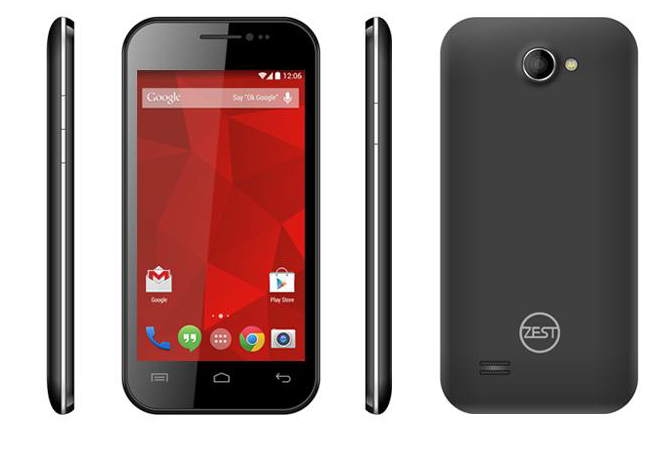
\includegraphics[width=1\linewidth]{./pictures/linphone.jpeg}
\caption{\label{fig:Linphone}3 of our members have been provided with a Zest T1 Android phone.}
\end{figure}
\end{center}

\newpage

%--------------------FunReq Create---------------------------s

\section{Introduction}

\subsection{Purpose}
\textbf{Description:}The purpose of this project is to extend Linphone's Instant Messaging (IM) implementation on Android platforms to include group chat and to implement other minor improvements to Linphones IM capabilities and user interface.
This project will give the student group exposure to:   
 \begin{itemize}
	\item Android development (Java and C)
	\item Open source contribution
	\item Cryptography
	\item Session initiation protocol (SIP)
	\item DO-178 certification
\end{itemize}
This project also forms part of a larger Masters study on development methodologies for projects seeking DO-178 certification.

\subsection{Scope}
\textbf{Description:}We are required to develop the following functionality for the Linphone project   
 \begin{itemize}
	\item Group chat (Invite additional members to a chat, all members receive chats)
	\item Secure group chat (AES256)
		\begin{itemize}
			\item A basic message encryption implementation will be provided
		\end{itemize}		 
	\item Creation and deletion of groups
	\item Voice record and send over IM
	\item Rework the messaging user interface
		\begin{itemize}
			\item Spacing between words are terrible
			\item Make the text bigger
			\item Block indents required to better specify who said what
			\item Presence indication to show a remote user is typing
			\item User picture portraits
		\end{itemize}		
\end{itemize}
\newpage

\section{Documentation conventions}
\textbf{Description:}DO-178B does not specify the documentation standard to be followed, but most projects do follow some or other documentation standard. The following figure is loosely based on MIL-STD-490A, although sometimes �Detail design� and �Notes� are changed into some other topic of discussion.\\


\begin{figure}
\centering
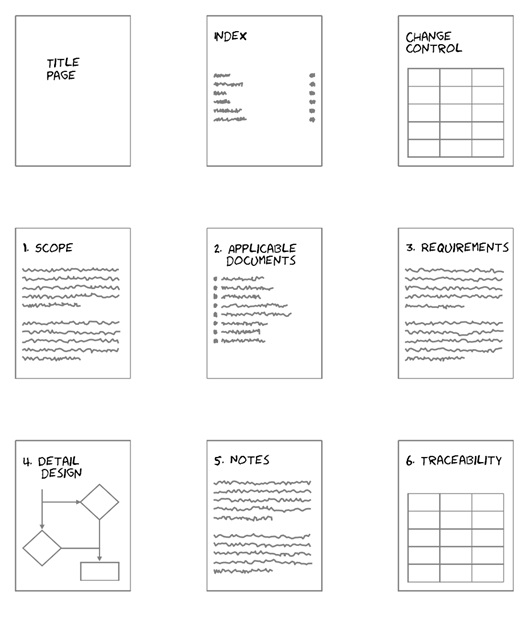
\includegraphics[width=1\linewidth]{./pictures/image1.jpg}
\caption{\label{fig:Agile}Agile development.}
\end{figure}

In the documentation, especially when talking about requirements and specifications, certain words convey additional meaning apart from their linguistic use. These words are usually capitalized.\\
\textbf{SHALL} and \textbf{SHALL NOT} - Indicates a mandatory requirement.
\textbf{WILL} and \textbf{WILL NOT} - Indicates a declaration of purpose or an expression of simple futurity.
\textbf{SHOULD} and \textbf{SHOULD NOT} - Indicates a non-mandatory desire, preference or recommendation.
\textbf{MAY} and \textbf{MAY NOT} - Indicates a non-mandatory suggestion or permission.
\textbf{MUST} and \textbf{MUST NOT} should be avoided as it causes confusion with the above terms. \\
\newpage

\section{System overview}
\subsection{Server Architecture}
%-----------------------Edit this section--------------------------
\newpage

\section{System overview}
\subsection{Software Architecture}
%-----------------------Edit this section--------------------------
\newpage


\section{Certification considerations}
The project will be developed according to DO-178 certification requirements, for level D certification. Justification for level D is not dependant on safety considerations as is usually the case, but rather on limited time and the limited experience the team has with DO-178.\\
This project is not intended for avionics applications and is not safety critical, but rather serves as a case study on DO-178 software development.\\
\newpage

\section{Software lifecycle}
An agile software development methodology will be followed with this project:\\

\begin{figure}
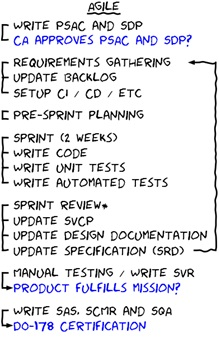
\includegraphics[width=1\linewidth]{./pictures/agile.jpg}\\
\caption{\label{fig:Agile}Agile development.}
\end{figure}
\newpage
%-------------------------

\subsection{Scrum}
During sprint planning and review sessions, we can review and update the Design Description (DD) document detailing the software architecture. At the end of a sprint, the implemented user stories will form the Software Requirements Data (SRD's). It will look something like this:\\

\begin{figure}
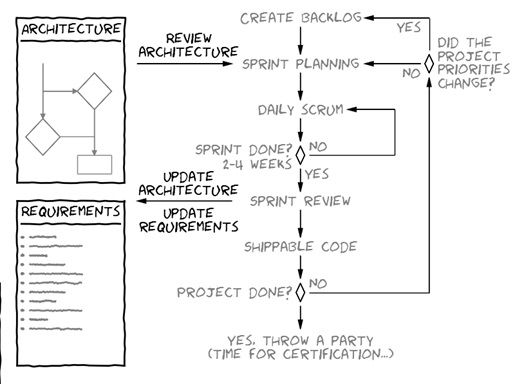
\includegraphics[width=1\linewidth]{./pictures/scrum.jpg}\\
\caption{\label{fig:Scrum}Scrum outputs.}
\end{figure}


During sprint planning we ensure that the user stories i.e. the high level requirements we are planning to implement is consistent with previous implemented requirements. During sprint review we update the requirements with the implemented user stories, and ensure the created functional tests and unit tests i.e. the low level requirements are consistent with the high level requirements (user stories).
\newpage

%-------------------------

\subsection{Continuous integration (CI) and Continuous deployment (CD)}

The CI and CD servers themselves are effectively the Software Life Cycle Environment Configuration Index (SECI), Software Configuration Index (SCI) and parts of the Sofware Configuration Management Records (SCMR) deliverables. For this to be possible, the CI server must have a copy of the version control database when duplicated for certification. \\
This means an agile setup might look as follows: \\

\begin{figure}
\centering
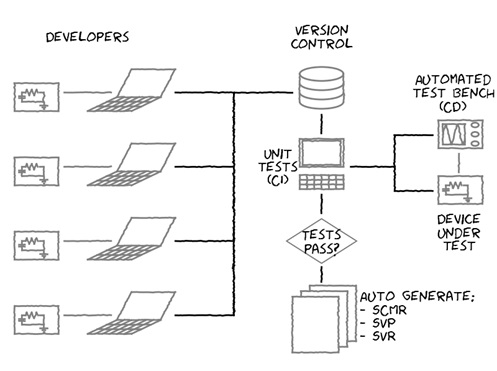
\includegraphics[width=1\linewidth]{./pictures/CI-CD.jpg}\\
\caption{\label{fig:Output}CI and CD outputs.}
\end{figure}


If all the tests pass, the CI / CD will autogenerate a snapshot of itself (VM�s or some other duplication means) and the version control database to serve as the SECI and SCI. It will also generate reports of the tests run and their results to serve as the SVP and SVR�s, and generate reports that can serve as SCMR items (This is baselines, commit histories etc.).
\newpage


%-------------------------
\subsection{Test driven development}
Test driven development can be used to generate the large parts of the Software Verification Cases and Procedures (SVCP�s) and Software Verification Results (SVR�s). High level requirements will be developed and tested with feature driven development, and unit tests will be used to develop and test low level requirements. But not all unit tests are really low level requirements, for instance testing if a function can handle null pointer parameters. As such we will mark which unit tests are indeed low level requirements in the unit testing code itself.\\ 
The relationship between the Continuous integration (CI) server and the Continuous deployment (CD) server is detailed in the popular test pyramid developed by Mike Cohn, where the CI is responsible for making sure the source code compiles at all times, and passes all unit tests, and the CD is responsible for making sure the automated functional tests pass at all times. One would expect to develop a lot more unit tests than functional tests, thereby limiting (but not eliminating) the need for expensive manual testing.\\
\newpage

%-------------------------

\section{Software development environment}

We will improve and revolve this sections out when we are comfortable in the project with the development environment.

\begin{itemize}
	\item Eclipse IDE
	\item Linux environment
	\item Java for user interface
	\item C for group chat functionalities
	\item Unit testing user interface
\end{itemize}
\newpage

%-------------------------

\section{Software lifecycle data}

The following deliverables will be created during this project:

\begin{itemize}
	\item \textbf{Plan for Software Aspects of Certification (PSAC)}\\
		The Plan for Software Aspects of Certification is the primary means used by the certification authority for determining whether an applicant is proposing a software life cycle that is commensurate with the rigor required for the level of software being developed.
	\item \textbf{Software Development Plan (SDP)}\\
		The Software Development Plan includes the objectives, standards and software life cycle(s) to be used in the software development processes.
	\item \textbf{Software Verification Plan (SVP)}\\
		The Software Verification Plan is a description of the verification procedures to satisfy the software verification process objectives.
	\item \textbf{Software Requirements Data (SRD)}\\
		Software Requirements Data is a definition of the high-level requirements including the derived requirements.
	\item \textbf{Software Design Description (SDD)}\\
		The Design Description is a definition of the software architecture and the low-level requirements that will satisfy the software high-level requirements.
	\item \textbf{Source Code}\\
		This data consists of code written in source language(s) and the compiler instructions for generating the object code from the Source Code, and linking and loading data. This data should include the software identification, including the name and date of revision and/or version, as applicable.
	\item \textbf{Executable Object Code}\\
		The Executable Object Code consists of a form of Source Code that is directly usable by the central processing unit of the target computer and is, therefore, the software that is loaded into the hardware or system.
	\item \textbf{Software Verification Cases and Procedures (SVCP)}\\
		Software Verification Cases and Procedures detail how the software verification process activities are implemented.
	\item \textbf{Software Verification Results (SVR)}\\
		The Software Verification Results are produced by the software verification process activities.
	\item \textbf{Software Accomplishment Summary (SAS)}\\
		The Software Accomplishment Summary is the primary data item for showing compliance with the Plan for Software Aspects of Certification.
\end{itemize}
%-------------------------

\section{Schedule / Software development plan}
The automated testing, setup of the CI and CD environment as well as the sprint back log will be implement and completed from the 22 June 2015 to the 5 July 2015 because that is when we conclude our exams and start implementations.
Please note that for each �story� we will setup unit testing and automated testing as discussed later on in the user role table.

\subsection{Task Description}

\begin{figure}
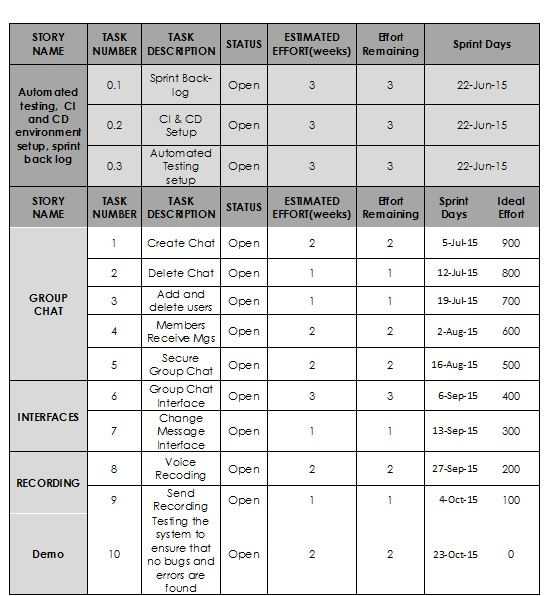
\includegraphics[width=1\linewidth]{./pictures/task.jpg}\\
\caption{\label{fig:Discription}Task Description.}
\end{figure}

\subsection{User Role}
Each task in the user story is implemented concurrently and sequentially as needed.

\begin{figure}
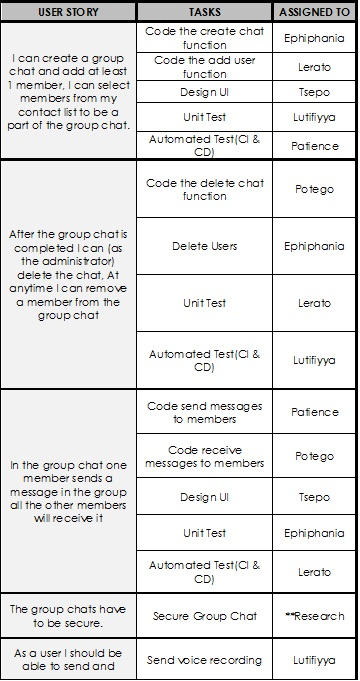
\includegraphics[width=1\linewidth]{./pictures/role.jpg}\\
\caption{\label{fig:Discription}Task Description.}
\end{figure}

\subsection{Burn Down Chart}

\begin{figure}
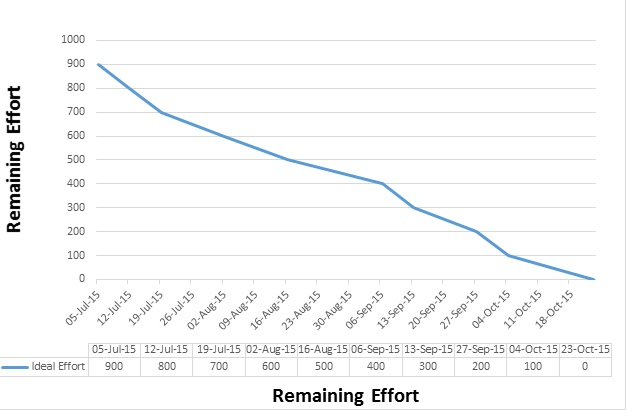
\includegraphics[width=1\linewidth]{./pictures/burnDown.jpg}\\
\caption{\label{fig:Discription}Task Description.}
\end{figure}
%-------------------------

\section{Licencing and ownership}
The aim is to open-source the project which would be published on Github as forked from Linphone project. 
\end{document}